\documentclass[pdftex,12pt,a4paper]{article}

\usepackage{graphicx}  
\usepackage[margin=2.5cm]{geometry}
\usepackage{breakcites}
\usepackage{indentfirst}
\usepackage{pgfgantt}
\usepackage{pdflscape}
\usepackage{float}
\usepackage{epsfig}
\usepackage{epstopdf}
\usepackage[cmex10]{amsmath}
\usepackage{stfloats}
\usepackage{multirow}


\renewcommand{\refname}{REFERENCES}
\linespread{1.3}

\usepackage{mathtools}
%\newcommand{\HRule}{\rule{\linewidth}{0.5mm}}
\thispagestyle{empty}
\begin{document}
\begin{titlepage}
\begin{center}
\textbf{}\\
\textbf{\Large{ISTANBUL TECHNICAL UNIVERSITY}}\\
\vspace{0.5cm}
\textbf{\Large{COMPUTER ENGINEERING DEPARTMENT}}\\
\vspace{2cm}
\textbf{\Large{BLG 222E\\ COMPUTER ORGANIZATION\\ PROJECT 2 REPORT}}\\
\vspace{2.8cm}
\begin{table}[ht]
\centering
\Large{
\begin{tabular}{lcl}
\textbf{PROJECT NO}  & : & 2 \\
\textbf{PROJECT DATE}  & : & 25.05.2022 \\
\textbf{GROUP NO}  & : & G29 \\
\end{tabular}}
\end{table}
\vspace{1cm}
\textbf{\Large{GROUP MEMBERS:}}\\
\begin{table}[ht]
\centering
\Large{
\begin{tabular}{rcl}
150190091  & : & Cemalettin Celal TOY\\
150190087  & : & Baran ISIK\\
150190084  & : & Mert Can ARABACI \\
\end{tabular}}
\end{table}
\vspace{2.8cm}
\textbf{\Large{SPRING 2022}}

\end{center}

\end{titlepage}

\thispagestyle{empty}
\addtocontents{toc}{\contentsline {section}{\numberline {}FRONT COVER}{}}
\addtocontents{toc}{\contentsline {section}{\numberline {}CONTENTS}{}}
\setcounter{tocdepth}{4}
\tableofcontents
\clearpage

\setcounter{page}{1}

\section{INTRODUCTION }
In this project, we implement a hardwired control unit for basic processor we designed in project1. This hardwired control unit consists of sequence counter, combinational control unit, 2 decoders and ALUSystem. Sequence counter, combinational control unit, 2 decoders recognize the instructions and create appropriate control signal for ALUSystem. Then ALUSystem performs operationsi such BRA, LD, ST, MOV, AND, OR, NOT, ADD, SUB, LSR, LSL, PUL, PSH, INC, DEC and BNE according to control signals.
\section{INSTRUCTIONS}
\begin{itemize}
    \item OPCODE (HEX) : \textbf{0x00}
    \begin{itemize}
        \item Symbol : BRA
        \item Addressing Mode : IM 
        \item Description : PC ← Value, we directly put the value of IR[7-0] to the PC due to addressing mode is immediate.
    \end{itemize}
    \item OPCODE (HEX) : \textbf{0x01}
        \begin{itemize}
            \item Symbol : LD
            \item Addressing Mode : IM, D
            \item Description : Rx ← Value, we put the value of M[AR] or IR[7-0] (due to its addressing mode is both D and IM) to the Rx to make the load.
        \end{itemize}
    \item OPCODE (HEX) : \textbf{0x02}
        \begin{itemize}
            \item Symbol : ST
            \item Addressing Mode : D
            \item Description : Value ← Rx, we put Rx to the M[AR] to make the store operation.
        \end{itemize}    
    \item OPCODE (HEX) :  \textbf{0x03} 
        \begin{itemize}
            \item Symbol : MOV
            \item Addressing Mode : N/A
            \item Description : DESTREG ← SRCREG1, we move source register 1 to destination register.
        \end{itemize}    
    \item OPCODE (HEX) : \textbf{0x04} 
        \begin{itemize}
            \item Symbol : AND
            \item Addressing Mode : N/A
            \item Description : DESTREG ← SRCREG1 AND SRCREG2, we make AND operation between source register 1 and 2 and put the result of it to destination register.
        \end{itemize}    
    \item OPCODE (HEX) :  \textbf{0x05} 
        \begin{itemize}
            \item Symbol : OR
            \item Addressing Mode : N/A
            \item Description : DESTREG ← SRCREG1 OR SRCREG2, we make OR operation between source register 1 and 2 and put the result of it to the destination register.
        \end{itemize}    
    \item OPCODE (HEX) :  \textbf{0x06}
        \begin{itemize}
            \item Symbol : NOT
            \item Addressing Mode : N/A
            \item Description : DESTREG ← NOT SRCREG1, we take complement of source register 1 and put the result of it to the destination register.
        \end{itemize}    
    \item OPCODE (HEX) : \textbf{0x07}
        \begin{itemize}
            \item Symbol : ADD
            \item Addressing Mode : N/A
            \item Description : DESTREG ← SRCREG1 + SRCREG2, we add source register2 to source register1 and put the result of it to  the destination register.
        \end{itemize}   
    \item OPCODE (HEX) : \textbf{0x08}
        \begin{itemize}
            \item Symbol : SUB
            \item Addressing Mode : N/A
            \item Description : DESTREG ← SRCREG2 - SRCREG1, we subtract source register2 from source register1 and put the result of it to  the destination register.
        \end{itemize}    
    \item OPCODE (HEX) : \textbf{0x09} 
        \begin{itemize}
            \item Symbol : LSR
            \item Addressing Mode : N/A
            \item Description : DESTREG ← LSL SRCREG1, we make logical shift left operation to source register1 and put the result of it to  the destination register.
        \end{itemize}    
    \item OPCODE (HEX) : \textbf{0x0A}
        \begin{itemize}
            \item Symbol : LSL
            \item Addressing Mode : N/A
            \item Description : DESTREG ← LSR SRCREG1, we make logical shift right operation to source register1 and put the result of it to  the destination register.
        \end{itemize}    
    \item OPCODE (HEX) : \textbf{0x0B}
        \begin{itemize}
            \item Symbol : PUL 
            \item Addressing Mode : N/A
            \item Description : M[SP] ← Rx; SP ← SP - 1, we put Rx to the M[SP] and decrease SP by 1.
        \end{itemize}    
    \item OPCODE (HEX) : \textbf{0x0C}  
        \begin{itemize}
            \item Symbol : PSH
            \item Addressing Mode : N/A
            \item Description :SP ← SP + 1; Rx ← M[SP], firstly we increase SP by 1 and then put M[SP] to the Rx.
        \end{itemize}    
    \item OPCODE (HEX) : \textbf{0x0D}
        \begin{itemize}
            \item Symbol : INC
            \item Addressing Mode : N/A
            \item Description : DESTREG ← SRCREG1 + 1, we increase source register1 by 1 and put the result of it to  the destination register.
        \end{itemize}    
    \item OPCODE (HEX) : \textbf{0x0E}
        \begin{itemize}
            \item Symbol : DEC
            \item Addressing Mode : N/A
            \item Description : DESTREG ← SRCREG1 - 1, we decrease source register1 by 1 and put the result of it to  the destination register.
        \end{itemize}    
    \item OPCODE (HEX) : \textbf{0x0F}
        \begin{itemize}
            \item Symbol : BNE
            \item Addressing Mode : IM
            \item Description : IF Z = 0 THEN PC ← Value, if Z is equal to zero then we put IR[7-0] to the PC (due to its addressing mode is immediate).
        \end{itemize}   
    \end{itemize}
    
\section{IMPLEMENTATION} 
\subsection{Hardwired Control Unit}
Our hardwired control unit has multiple modules. There are ALUSystem that we created in project1, Sequence Counter and Combinational Control Unit . ALUSystem fetches instructions from memory to the Instruction Register. A decoder with 4 bit selection inputs decodes Instruction Registers 15-12 bits which is the OpCode part and sends output signals to combinational control unit. Also there is a sequence counter, which count from 0 to 7, in order to perform operation at appropriate clock signals. A decoder with 3 bit selection inputs, decodes T coming from sequence counter and sends T0, T1, T2, ...., T7 signals to combinational control unit. Inside combinational control unit, all of the control signals that will be sent to ALUSystem is determined according to T, OpCode, SRCREG1, SRCREG2, DESTREG signals. Lastly, outputs of combinational circuit is sent to ALUSystem to perform instructions.
\begin{figure}[ht]
	\centering
	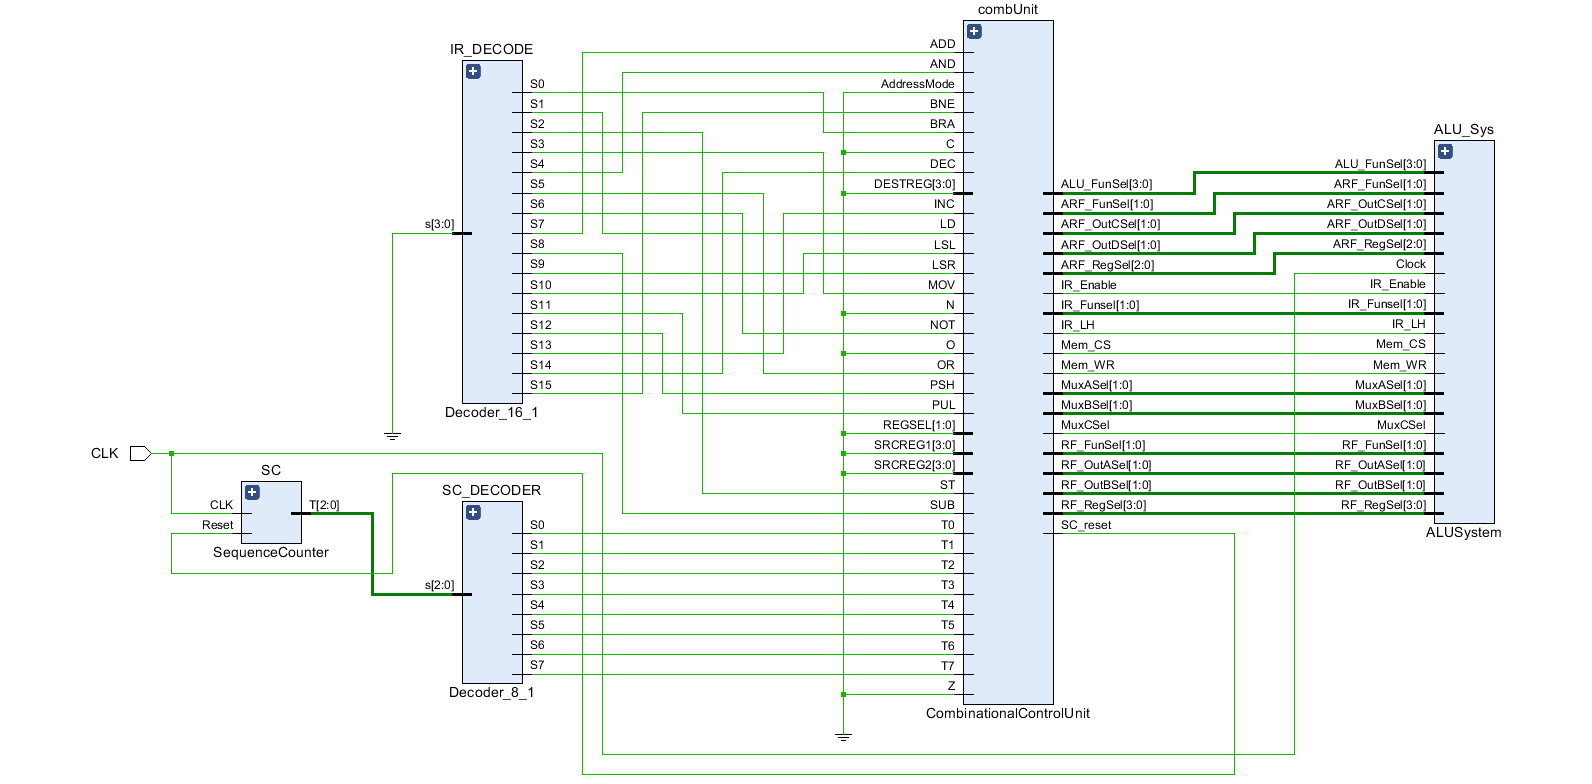
\includegraphics[width=1\textwidth]{Hardwired Control Unit.png}	
	\caption{Hardwired Control Unit}
	\label{fig1}
\end{figure}
\subsection{Sequence Counter}
Sequence counter generates timing signals which will control clock cycle for micro-operations. Timing signals will be sent to combinational circuit and used while arranging the control signals for ALUSystem. When an instruction is completed. Reset signal is sent to sequence counter and timing signal reset to T0.
\begin{figure}[ht]
	\centering
	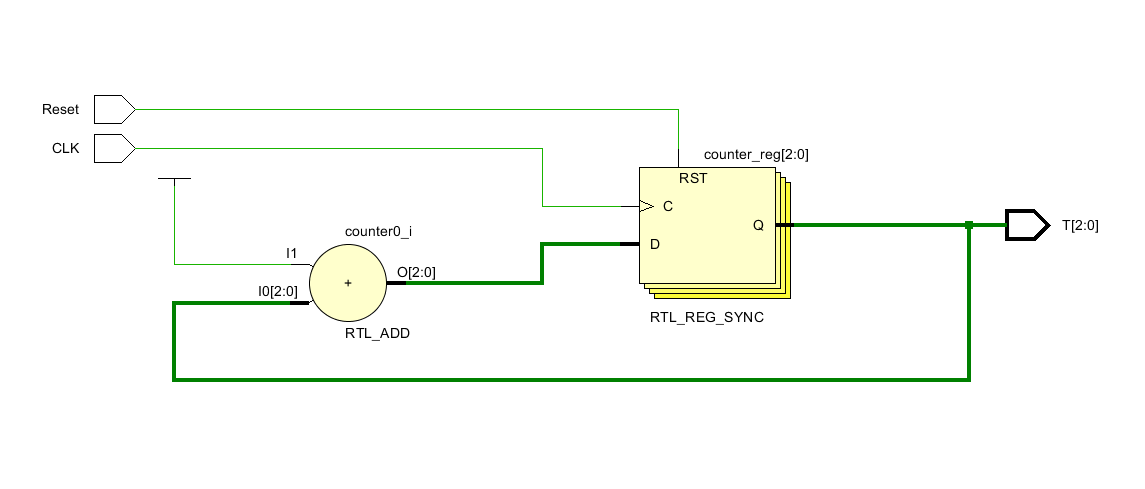
\includegraphics[width=1\textwidth]{sequence counter.png}	
	\caption{Sequence Counter}
	\label{fig1}
\end{figure}
\subsection{Combinational Control Unit}
Combinational control unit takes T signals, OpCode signal from decoder, REGSEL, DESTREG, SRCREG1, SRCREG2, AddressMode from instruction register of ALUSystem and Z, C, N, O from ZCNO flag register of ALUSystem as inputs. Then according to these inputs , it sets control signals for corresponding instructions and sends them to ALUSystem.   
\subsubsection{RESET}
When our basic computer is initiated, all of our registers are empty and we need to reset them. At the initiation, sequence counter starts counting from T7. That's because we use 1 clock cycle in order to reset all of the registers. Then it becomes T0. Since we don't reach T7 in any instruction in our basic computer, sequence counter sends T7 signal only 1 time.
\subsubsection{FETCH}
Fetch operation is completed in 2 clock cycles because the data we take from memory is 8 bit but our instructions are consist of 16 bits. At T0 MemCS and MemWR are set to 0 in order to read from memory. IR is enabled and IRLH 1 becuase we load the data from memory to IR(7-0). Then we increment the PC by 1. At T1, MemCS and MemWR are set to 0 and IR is enabled again but this time IRLH is 0 because we load the data from memory to IR(15-8) and complete the fetch operation. Each time we load data from memory to instruction register, we increment PC by 1. After fetch operation, data inside instruction register is decoded and sent to combinational control unit.
\subsubsection{BRA, BNE}
BRA and BNE operations is completed in 1 clock cycle. In these instructions, we set MuxBSel to 00 at time T2 so that IROut(0-7) comes as Include bits of Address Register File. Moreover, we set ARFFunSel to 10, and ARFRegSel to 011 in order to load to PC at time T2. we make other registers disable. Finally, we reset the clock cycle thanks to SC-reset. Even though both instructions perform same operations, there is a difference. For BNE instruction, operations explained in the paragraph are performed only when Z flag inside ZCNO register is 0. Otherwise BNE instruction does nothing
\subsubsection{LD}
LD operation is completed in 1 clock cycle. In this operation, when address mode of IR is 0, we set ARF-OutDSel to 10 so that AR comes as Address bits of Memory. In addition, we set Mem-WR to 0, and Mem-CS to 0 for reading mode of memory. We set MuxASel to 01 at time T2 so that Memory Output comes as Include bits of Register File.
When address mode of IR is 1, we set MuxASel to 00 at time T2 so that IROut(0-7) comes as Include bits of Register File.
In both situations, We must set RF-FunSel to 10 for the loading. Also we choose the register thanks to REGSEL bits of IR.
Finally, we reset the clock cycle thanks to SC-reset.
\subsubsection{ST}
ST operation is completed in 1 clock cycle. In this operation, We did all the operations at the time of T2. We sent the value of the selected register from the OutB of the register file and passed it over to the ALU to make it go through the memory. Thus, we set RF-OutBSel to REGSEL bits of IR, and ALU-FunSel to 0001. In order to writing the incoming value to M[AR], we set ARF-OutDSel to 10. Moreover, we set Mem-WR to 1, and Mem-CS to 0 for writing mode of memory.Finally, we reset the clock cycle thanks to SC-reset.
\subsubsection{MOV}
MOV operation is completed in 1 clock cycle. In this operaiton, we make destination register enable thanks to DESTREG. Then, we sent the value in the source register to the appropriate output. For loading, we set the funsel of register to 10( if DESTREG[2s=0, ARF-FunSel,else if. When SRCREG[2] is 0, we set MuxASel or MuxBSel to 10, and 11 respectively. On the other condition, we set MuxASel or MuxBSel to 11, and 11 respectively. We set FunSel of register file or Address register file to load mode according to DESTREG. Finally, we reset the clock cycle thanks to SC-reset.
\subsubsection{ALU operations (AND, OR, NOT, ADD, SUB, LSR, LSL)}
These instructions will be completed in 1 clock cycle, but SUB instruction will be completed in 3 clock cycles. Due to the internal structure of the ALU, sometimes we need to make SRCREG1 - SRCREG2 instead of SRCREG2 - SRCREG1. In order to correct this confusion, the complement of the SUB operation is calculated at the time of T3 and 1 is added to this calculated value at the time of T4. In these operations, we make destination register enable thanks to DESTREG. Then, we sent the value in the source register to the appropriate outputs. We routed these outputs to the A and B inputs of the ALU according to each operation. When DESTREG[2] is 0, we set ARF-FunSel to 10. When DESTREG[2] is 1, we set RF-FunSel to 10. Finally, we reset the clock cycle thanks to SC-reset.
\subsubsection{PUL}
This instruction will be completed in 2 clock cycles. At T2, we increment the SP register. For incrementation, we arrange ARFRegSel as 110 and ARFFunSel as 01. Since we don't have any work to do with IR, RF and memory, we disable them by giving IREnable 0, RFRegSel 1111 and MemCS 1. Also reset input for sequence counter is 0, because the instruction is not completed. For T3, we give ARFOutDSel 11 because SP needs to be given as address to memory, rMemWR 0 and rMemCS to be able to read from memory. Then we arrange RFRegSel and ARFRegSel according to DESTREG. If DESTREG[2] is 1, it means that destination register is in RF. Thus we give ARFRegSel 111, RFFunSel 10 (because we will load), MuxASel 01 (because data coming from memory output) and defined RFRegSel according to DESTREG[1:0]. If DESTREG[2] is 0, it means that destination register is in ARF. Thus we give RFRegSel 1111, ARFFunSel 10 (because we will load), MuxBSel 10 (because data coming from memory output)and defined ARFRegSel according to DESTREG[1:0].
Since the instruction will be completed at the end of T3, we give SCReset 1.
\subsubsection{PSH}
PSH instruction can be completed in 1 cycle. At T2, we make MemCS 0 and MemWR 1 to write the data to memory, ARFOutDSel 11 to give SP to memory as address, ARFRegSel 110 and ARFFunSel 00 to increment the SP register. Since giving SP from ARF to memory and incrementing SP will be at the same cycle, the address given to the memory will be SP before the incrementation. Also, if SRCREG1 is a register inside ARF, we give MuxCSel 0, ARFOutCSel SRCREG1[1:0] and ALUFunSel 0000, because data needs to be carry from ARF to MuxC, from MuxC to ALU and from ALU to memory. if SRCREG1 is a register inside RF, we give MuxCSel 1, RFOutASel SRCREG1[1:0] and ALUFunSel 0000, because data needs to be carry from RF to MuxC, from MuxC to ALU and from ALU to memory.

\subsubsection{INC, DEC}
INC and DEC operation will be completed in two clock cycles. When the fist clock cycle(T2) comes, the value of SRCREG is send to DESTREG. When the second clock cycle(T3) comes, the value of DESTREG is increased. In these operations, we make destination register enable thanks to DESTREG. Then, we sent the value in the source register to the appropriate output. For loading, we set the funsel of register to 10 (if DESTREG[2]=0, ARF-FunSel, else if DESTREG[2]=1, RF-FunSel). At the next clock signal, we set the funsel of register to 00(Decrement) or 10(Increment) for decrement or increment. Finally, we reset the clock cycle thanks to SC-reset. Also, we carried the data after incrementation or decrementation to ALU in order to check if flags in ZCNO register changes.

\newpage
\section{DISCUSSION AND RESULTS} 
While implementing project, first of all, we design the SequenceCounter module for clock cycle. Then, we decode the result of SequenceCounter with 1 to 8 decoder. Also, we use a 1 to 16 decoder in order to decode the IR.
Secondly, we design the CombinationalControlUnit module. This module is responsible for determining the inputs of the ALU system, which we made in the previous project, according to the clock signal and OPCODE.
Finally, we design the HardwiredControlUnit module. In this module, we make all connections between the ALU system, SequenceCounter, CombinationalControlUnit and decoders.

For the project, we were given a RAM.mem file and a example code in pdf. The example code adds the data at the 0xA0, 0xA1, 0xA2, 0xA3, 0xA4 memory addresses and stores the result in address 0xA6. According to this code, we write appropriate data to correct addresses of memory and run our module. Our basic is initiated, all registers are reset. That's why, at fetch time, it loads the data that is stored at memory address 0x00 and incremented.
\begin{itemize}
    \item BRA 0x20
    \begin{itemize}
       \item The first instruction is BRA. After its fetch operation is completed, IR(7-0) is sent to PC register at T2 and clock resets.
        \begin{center}
            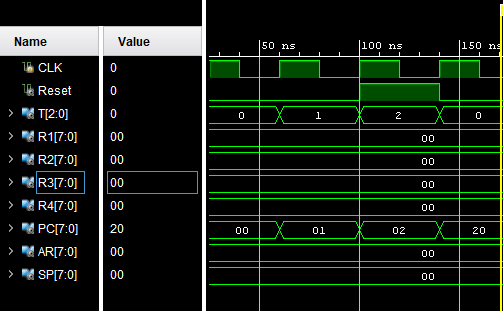
\includegraphics[width=0.6\textwidth]{BRA.png}	\newline
        \end{center}
    \end{itemize} 
    \item LD R1 IM 0x05
    \begin{itemize}
        \item At T2, it loads 0x05 to R1 register, which will be used as iteration counter.
        \begin{center}
            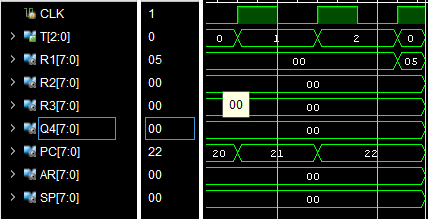
\includegraphics[width=0.6\textwidth]{LD R1 IM.png}	\newline
        	\label{fig1}
        \end{center}
    \end{itemize}
    \item LD R2 IM 0x00
    \begin{itemize}
        \item At T2, it loads 0x00 to R2 register, which will store total result.
        \begin{center}
            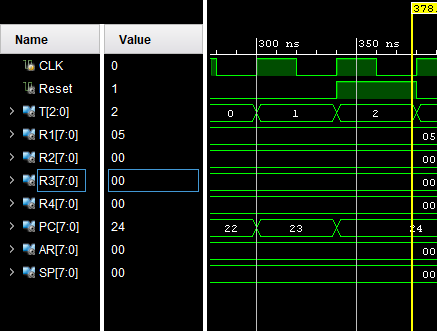
\includegraphics[width=0.6\textwidth]{LD R2 IM 0x00 .png}\newline
        	\label{fig1}
        \end{center}
    \end{itemize}
    \item LD R3 IM 0xA0
    \begin{itemize}
        \item At T2, it loads 0xA0 to R3 register.
        \begin{center}
            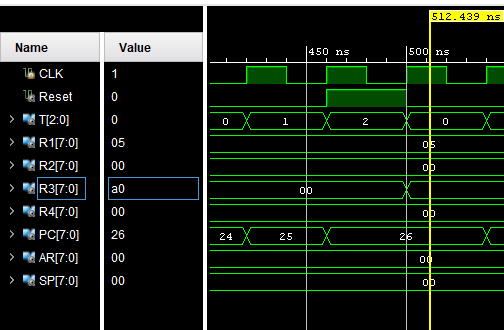
\includegraphics[width=0.6\textwidth]{LD R3 IM 0xA0.png}\newline
        	\label{fig1}
        \end{center}
    \end{itemize}
    \item MOV AR R3
    \begin{itemize}
        \item At T2, it moves the data inside R3 to AR register.
        \begin{center}
            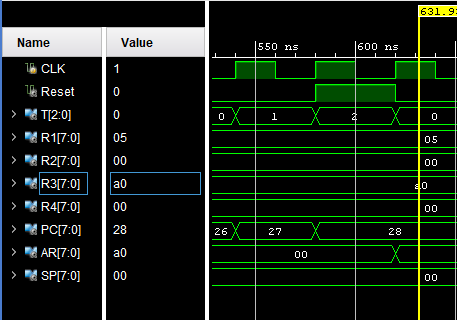
\includegraphics[width=0.6\textwidth]{MOV AR R3 .png}\newline
        	\label{fig1}
        \end{center}
    \end{itemize}
    \item LD R3 D
    \begin{itemize}
        \item At T2, it loads the data located in M[AR] to R3 register.
        \begin{center}
            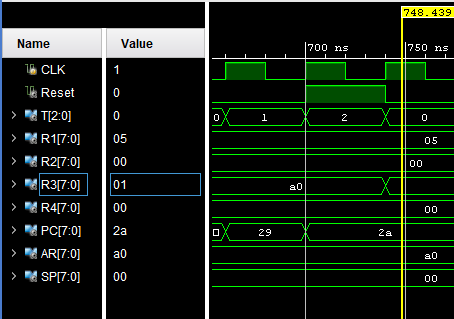
\includegraphics[width=0.6\textwidth]{LD R3 D.png}\newline
        	\label{fig1}
        \end{center}
    \end{itemize}
    \item ADD R2 R2 R3
    \begin{itemize}
        \item At T2, it adds the data inside R3, which is loaded in LD R3 D instruction, to R2.
        \begin{center}
            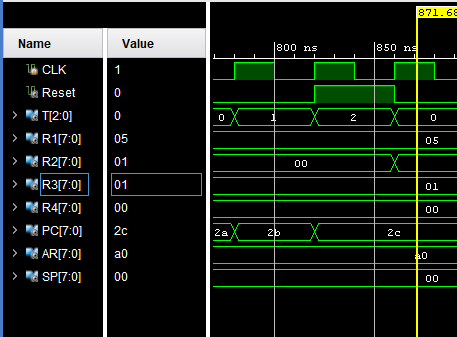
\includegraphics[width=0.6\textwidth]{ADD R2 R2 R3.png}\newline
        	\label{fig1}
        \end{center}
    \end{itemize}
    \item INC AR AR
    \begin{itemize}
        \item At T2, it increases AR register.
        \begin{center}
            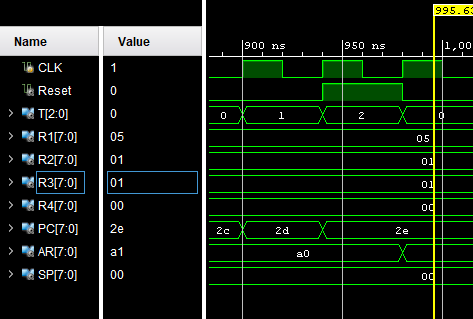
\includegraphics[width=0.6\textwidth]{INC AR AR.png}\newline
        	\label{fig1}
        \end{center}
    \end{itemize}
    \item DEC R1 R1
    \begin{itemize}
        \item At T2, it decreases R1 register, which means that once iteration is completed. If R1 register becomes 0 after decreasing, the program will start its last iteration and Z flag will be 0.
        \begin{center}
            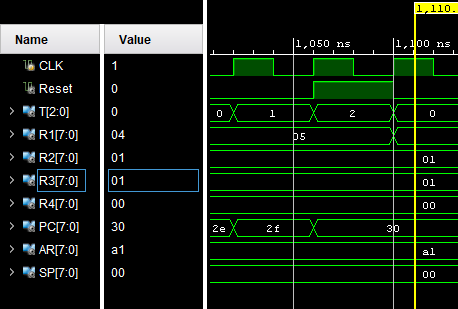
\includegraphics[width=0.6\textwidth]{DEC R1 R1.png}\newline
        	\label{fig1}
        \end{center}
    \end{itemize}
    \item BNE IM LABEL
    \begin{itemize}
        \item At T2, it checks if Z flag is 0 or not. If it is 0, it loads the address symbolized as 'LABEL' to PC register, which means our program will go back to LD R3 D instruction and start another iteration. If Z is 1, it does nothing and resets clock.
        \begin{center}
            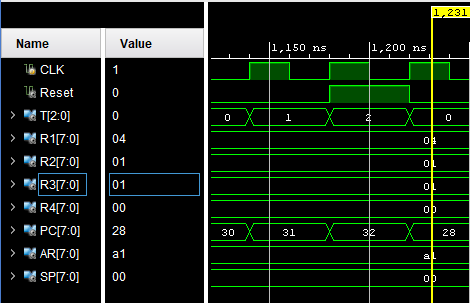
\includegraphics[width=0.6\textwidth]{BNE IM LABEL.png}\newline
        	\label{fig1}
        \end{center}
    \end{itemize}
    \item INC AR AR
    \begin{itemize}
        \item At T2, after iteration for summing all the data inside 0xA0, 0xA1, 0xA2, 0xA3, 0xA4 memory addresses finishes, AR is incremented once more and become 0xA6 
        \begin{center}
            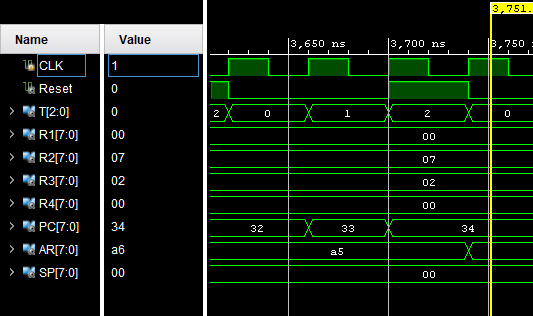
\includegraphics[width=0.6\textwidth]{INC AR AR2.png}\newline
        	\label{fig1}
        \end{center}
    \end{itemize}
    \item ST R2 D
    \begin{itemize}
        \item At T2, it writes the data inside R2 to M[AR], which is 0xA6 address of the memory.
        \begin{center}
            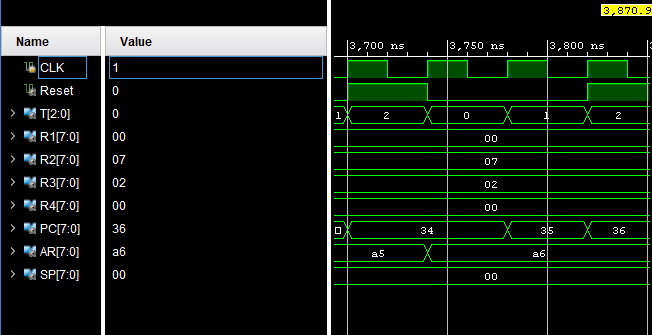
\includegraphics[width=0.6\textwidth]{ST R2 D.png}\newline
        	\label{fig1}
        \end{center}
    \end{itemize}
\end{itemize}  
As a result, 0xA6 address of the memory will have the result of our addition operation.
M[A0] + M[A1] + M[A2] + M[A3] + M[A4] = M[A6]
\begin{center}
    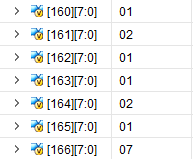
\includegraphics[width=0.4\textwidth]{result.png}\newline
    \label{fig1}
\end{center}

\section{CONCLUSION}
In this Project, we have learnt how a basic computer works and performs various instructions. First, we determined what inputs our ALUSystem needs to complete each instruction and how many clock cycle each instruction need. Then, we determined the conditions for each instruction to run and started to impelement our module. We created sequence counter for timing signal, decoder to decode IR and output of sequence counter and combinational control unit to set appropriate control signals for ALUSystem's inputs. Finally ALUSystem completed instructions. 
After we finished the project, we write our RAM file according example code in PDF and check the results. According to example code, we summed M[160](2'h01), M[161](2'h02), M[162](2'h01), M[163](2'h01), M[164](2'h02) and write the result 2'h07 to M[166].

\newpage
\end{document}

